\documentclass{standalone}
\usepackage{pgfplots}
%\usepackage{fontspec}
\usetikzlibrary{arrows,positioning}
% \setmainfont{xkcd}


\renewcommand{\familydefault}{\sfdefault}


\begin{document}


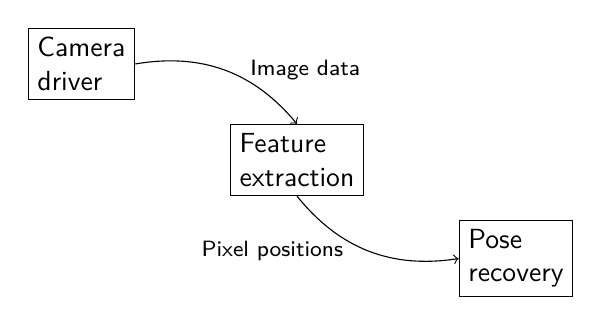
\begin{tikzpicture}[auto,decoration={random steps,segment length=1mm,amplitude=0.3pt}]
	
\node[draw,rectangle,align=left] (cam_driver) {Camera\\driver};


\node[draw,rectangle,below right=0.3cm and 1.2cm of cam_driver,align=left] (feat_ext) {Feature \\extraction};


\path[->] (cam_driver.east)  edge   [bend left]   node[above, right=0.2cm] {\footnotesize Image data} (feat_ext.north);


\node[draw,rectangle,below right=0.3cm and 1.2cm of feat_ext,align=left] (pose_rec) {Pose\\recovery};


\path[->] (feat_ext.south)  edge   [bend right]   node[below, left=0.2cm] {\footnotesize Pixel positions} (pose_rec.west);


\end{tikzpicture}


\end{document}